\chapter{Аналитическая часть}

В данном разделе описаны основные идеи алгоритма конвейерных
вычислений. Поставлена задача, для которой будет применяться этот
алгоритм в качестве примера\cite{example}.


\section{Описание алгоритма параллельной конвейерной об­работки данных}



Конвейер - способ организации вычислений, используемый в со­временных
 процессорах и контроллерах с целью повышения их произ­водительности
  (увеличения числа инструкций, выполняемых в единицу
времени — эксплуатация параллелизма на уровне инструкций).


На рисунке \ref{pic:parall-pipeline1} изображена схема, 
иллюстрирующая работу кон­вейера с параллельной реализацией.

\begin{figure}[!htb]
	\centering
	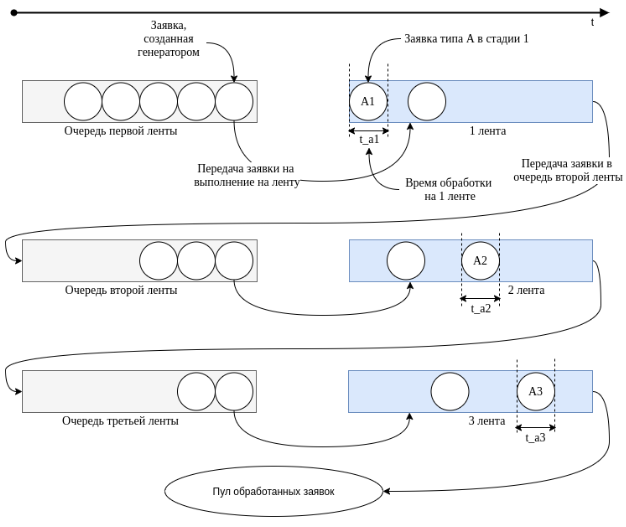
\includegraphics[scale=0.5]{imgs/1}
	\caption{Схема, иллюстрирующая работу конвейера с
	параллельной реализацией}
	\label{pic:parall-pipeline1}
\end{figure}


Рассмотрим, как заявка перемещается между разными лентами (\ref{pic:parall-pipeline2})

\begin{figure}[!htb]
	\centering
	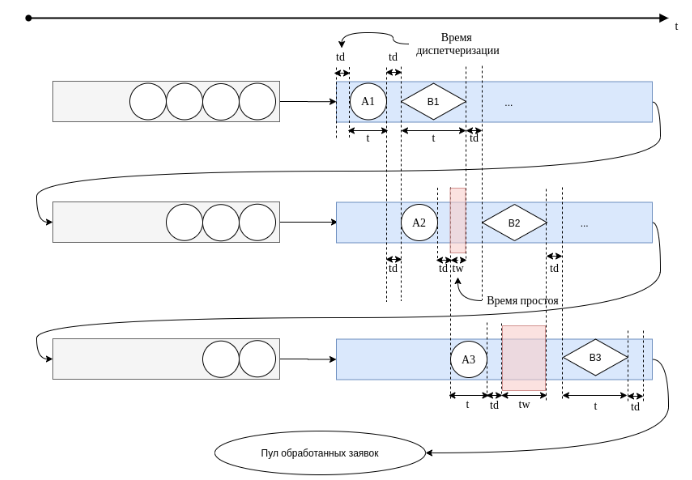
\includegraphics[scale=0.5]{imgs/2}
	\caption{Схема, иллюстрирующая пример работы конвейра с
	параллельной реализацией}
	\label{pic:parall-pipeline2}
\end{figure}


Время диспетчеризации (td) -- время, в течение которого заявка снимается/добавляется в очередь.

Время простоя (tw) -- время, которое тратится на ожидание заяв­ки.

По этому рисунку можно сделать вывод, что в зависимости от сложности заявок может 
сложиться такая ситуация, что лента будет про­стаивать.

Например, если две первые заявки более трудоемкие, чем третья, то третья заявка будет
 долго ждать обработки на других лентах, а кон­кретно до тех пор, пока не обработаются 
 первые две. Однако, если бы она была первой в очереди на обработку первой лентой, 
 то время простоя бы сократилось.

Лента ``живет'' в терминологии потока, пока либо не выполнит план, либо не получит 
сигнал о завершении работы.

Нельзя завершить задачу, пока она не обработана до конца, поэто­му, даже если
был получен сигнал о завершении, необходимо дождаться завершения выполнения
заявок, которые на момент получения сигнала находились в состоянии обработки.

Генератор заявок может быть статический или динамический. В случае статического 
очередь формируется заранее, в случае динамического -- очередь может формироваться 
в течение некого периода в зависимости от условий.

\section{Постановка и описание задачи для конвейерной об­работки}

В качестве алгоритма, реализованного для распределения на конвейере, было выбрана
реализация слегка видоизмененная версия команды Unix-подобной операционной системы \texttt{md5sum}. 

Данная команда позволяет вычислять значения хеш-сумм файлов по алгоритму MD5. В
обычном случае вычисленные хеши выводятся. В других случаях программа сверяет 
вычисленные значения со значениями, сохранёнными в файле. Наиболее часто программа 
используется для проверки правильной загрузки файлов по сети. 

Программа, релизуемая в рамках данной лабораторной работы программа похожа на 
\texttt{md5sum}, однако она принимает в качестве 
аргумента один каталог и печатает значения хеш-суммы для каждого файла в этом каталоге.

Таким образом, алгоритм работы программы состоит из 3-х этапов:

\begin{itemize}
	\item получение полного пути файла;
	\item вычисление хеш-суммы при помощи алгоритма MD5 содержимого файла;
	\item агрегирование полученных результатов и сохранение в результирующую структуру.
\end{itemize}


\section{Вывод}

В данном разделе были описаны основные идеи алгоритма парал­лельной 
конвейерной обработки данных, а также поставлена задача, для которой 
будет применяться этот алгоритм в качестве примера.

Входными данными для программного обеспечения являются:
\begin{itemize}
	\item путь к файлу или директории в файловой системе;
	\item количество потоков для вычисления хеш-суммы.
\end{itemize}

Выходными данными явлются:
\begin{itemize}
	\item список обработанных файлов и соответствующие им хеш–суммы;
	\item усредненные временные характеристики конвейера: среднее время обработки заявки 
	каждой из лент, а так же усредненное время ожидания в каждой из очередей конвейера.
\end{itemize}

На программное обеспечения накладываются следующие ограничения:
\begin{itemize}
	\item корректность входных данных;
	\item обладания соответствующими правами для чтения исходных файлов.
\end{itemize}